%

\newpage

\titulo{Notas metodológicas}


\noindent\textbf{Recopilación:}

La recopilación de los datos estadísticos de Seguridad Alimentaria y Nutricional (SAN) para el Compendio Estadístico SAN 2014 se llevó a cabo siguiendo los siguientes pasos:
\begin{itemize}
	\item[a.]	{\textbf{Identificación de indicadores y sub-indicadores} El primer paso para elegir los indicadores y sub-indicadores del Compendio fue llevar a cabo una revisión bibliográfica de la información sobre SAN disponible (INE, 2013; FAO, 2014; DevTech Systems, Inc., \& Iarna/URL, 2015; URL, Iarna, IICA, \& McGill University, 2015). Como resultado se obtuvo una lista de indicadores bastante amplio; sin embargo, se decidió reducir el número de indicadores para que la información fuese manejable. Esto se hizo con la ayuda de expertos en SAN, lo que dio como resultado el listado de indicadores y sub-indicadores final (Figura 4,  Figura 6, Figura 7, Figura 8, Figura 9 y Figura 10). El indicador y sub-indicadores de la dimensión 7 se agregaron con el fin de integrar los logros en SAN hasta la fecha. }

\item[b.]	\textbf{Cuestionarios en línea} El Iarna-URL, junto con el apoyo del personal del INE, elaboró cinco cuestionarios en el programa Surveymonkey. Los mismos contenían preguntas para llevar a cabo un diagnóstico de la información con la que las organizaciones productoras y recopiladoras de estadísticas de SAN contaban. Cada cuestionario corresponde a las dimensiones/pilares en las que se basa el Compendio. En un principio, se enviaron los cuestionarios únicamente a las instituciones miembros de la Oficina Coordinadora Sectorial de Estadísticas de Seguridad Alimentaria y Nutricional (Ocsesan) que contaran con información relacionada con los indicadores y sub-indicadores elegidos. No obstante, se envió el listado de indicadores y sub-indicadores a todas las instituciones miembros de la Ocsesan para que fueran ellas quienes determinaran si podían aportar información o no. Asimismo, se enviaron los cuestionarios a otras instituciones sugeridas por las instituciones miembros.


\item[c.]	\textbf{Diagnóstico de información por organización} Con base en los resultados del cuestionario, se realizaron cuadros resumen para conocer con qué información contaba cada institución, para así crear cuadros de salida tentativos y recopilar la información final del compendio.

\item[d.]	\textbf{Diseño de cuadros de salida} Para diseñar los cuadros de salida del Compendio, se llevaron a cabo cuatro reuniones extraordinarias de la Ocsesan, en las que participó personal del Iarna-URL, el INE y la Sesan. Se diseñaron cuadros para cada uno de los pilares/dimensiones del Compendio y se socializaron en la octava reunión de la Ocsesan celebrada en octubre de 2015. Los asistentes a dicha reunión evaluaron los cuadros y sugirieron cambios que luego se hicieron en otra reunión extraordinaria.

\item[e.]	\textbf{Recopilación de información en instituciones} La recopilación de información de datos fue llevada a cabo por dos técnicos contratados por el Iarna-URL, y personal de la Sesan, el INE y el Iarna-URL, quienes utilizaron las fuentes más recientes disponibles, y llenaron los cuadros de salida previamente elaborados. Durante este proceso fue que realmente se verificó la disponibilidad y calidad de la información. Los técnicos cambiaron en alguna medida los cuadros de salida, eliminando información en algunos casos, y enriqueciendo los cuadros en otros, dependiendo de la disponibilidad y calidad de la información estadística. A pesar de que la información para algunos de los indicadores no estaba disponible, o no presentaba la calidad requerida para formar parte del Compendio, se decidió dejar el listado de indicadores intacto, con el fin de conseguir la información en futuras versiones de este documento.
\end{itemize}


\noindent\textbf{Procesamiento y control de calidad:}

Se debe tomar en cuenta que la información presentada en cada una de las dimensiones es responsabilidad de cada fuente de información. Asimismo, se tomó en cuenta la información disponible más actualizada. La fuente de la información está indicada en la parte inferior de cada cuadro. 

\noindent\textbf{Integración:}

Se integraron los cuadros ya llenos en los respectivos capítulos del Compendio. 

\noindent\textbf{Edición y diagramación:}


Se editó el borrador final y se realizó la diagramación correspondiente para obtener un documento de calidad. Se tomaron datos de los cuadros integrados para la generación de gráficas.

\noindent\textbf{Revisión editorial, aprobación e impresión:}

Se integró un equipo para la revisión final del documento, conformado por personal del Iarna-URL y el INE. El informe se sometió a la aprobación de la Sección de Socieconómicas y Ambientales del INE, y finalmente se envió a imprenta.



%

\newpage

\titulo{Importancia de la seguridad alimentaria y nutricional}


\noindent\textbf{1. Seguridad alimentaria y nutricional a nivel mundial y regional:}

En el ámbito mundial y de acuerdo con estimaciones de la Organización de las Naciones Unidas para la Alimentación y la Agricultura (FAO, por sus siglas en inglés), se han logrado importantes avances para erradicar el hambre, incluyendo a los países en desarrollo, los cuales representan la gran mayoría de la subalimentación mundial. Se calcula que en en el período de 2012 a 2014, la población en países en desarrollo que padecía hambre crónica era de 791 millones de personas, es decir, 203 millones menos que en en el período de 1990 a 1992 (FAO, FIDA \& PMA, 2015). 

Según la FAO (2015a) «La seguridad alimentaria se da cuando todas las personas tienen acceso físico, social y económico permanente a alimentos seguros, nutritivos y en cantidad suficiente para satisfacer sus requerimientos nutricionales y preferencias alimentarias, y así poder llevar una vida activa y saludable».

La Cumbre Mundial sobre la Alimentación (CMA), se convocó como respuesta a la persistencia de una desnutrición generalizada y a la preocupación por la capacidad de la agricultura para cubrir las necesidades futuras de alimentación. En 1974, los gobiernos participantes en la Conferencia Mundial de la Alimentación proclamaron que «todos los hombres, mujeres y niños tienen derecho inalienable a no padecer de hambre y malnutrición a fin de poder desarrollarse plenamente y conservar sus facultades físicas y mentales». Además, la Conferencia se fijó el objetivo de erradicar el hambre, la inseguridad alimentaria y la malnutrición en el plazo de un decenio, objetivo que no se alcanzó (FAO, s.f.).  

Posteriormente, se llevó a cabo la Cumbre Mundial sobre la Alimentación, celebrada del 13 al 17 de noviembre de 1996. Los participantes fueron los representantes de 185 países y de la Comunidad Europea del Este. La misma constituyó un foro para el debate sobre una de las cuestiones más importantes con que se enfrentan los dirigentes mundiales: La erradicación del hambre (FAO, s.f).

El hambre, la inseguridad alimentaria y la nutrición son problemas complejos que no pueden ser resueltos por un solo sector. Es necesario tomar una serie de medidas en diversos sectores que aborden las causas inmediatas y subyacentes del hambre. Entre estos sectores se encuentran: la producción y productividad agraria, el desarrollo rural, la silvicultura, la pesca, la protección social, y el comercio y los mercados. Asimismo, la gobernanza de la seguridad alimentaria se refiere a fomentar un entorno propicio que cree incentivos para que los sectores involucrados mejoren su repercusión sobre el hambre, la malnutrición y la inseguridad alimentaria (FAO, FIDA \& PMA, 2015) (Figura \ref{figura1})

\begin{figure}
		\centering
	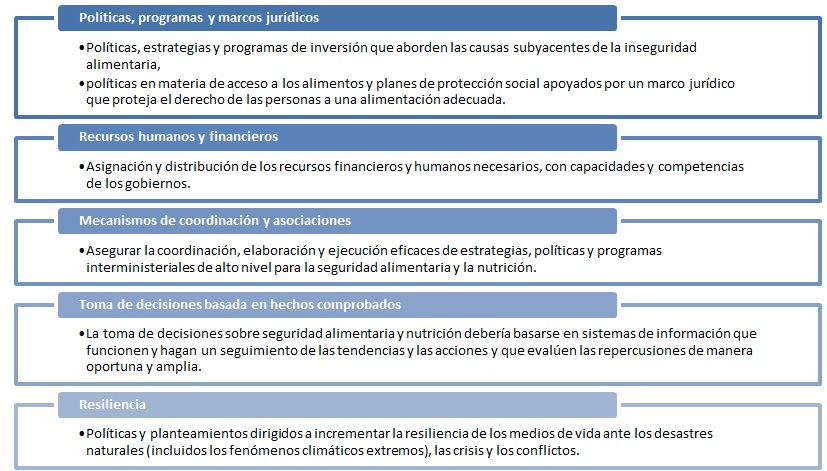
\includegraphics[width=0.7\textwidth]{figura1}
	\caption{Cinco dimensiones fundamentales de un entorno propicio para la gobernanza de la seguridad alimentaria y nutricional. \textbf{Elaborado por:} Iarna-URL, 2015 con base en FAO, FIDA \& PMA, 2015.}
	\label{figura1}
%	\centering
\end{figure}
%$\ $\\[-1cm]
Los estados latinoamericanos y caribeños tomaron la decisión de acabar con el hambre para 2025, fundamento para la acción nacional y regional de promover la seguridad alimentaria. La región en conjunto es la única que alcanzó la meta del primer Objetivo de Desarrollo del Milenio (ODM) relacionada con el hambre. Asimismo, América Latina alcanzó el objetivo de la Cumbre Mundial sobre la Alimentación (FAO, FIDA \& PMA, 2015). 


\noindent\textbf{2.	Seguridad alimentaria y nutricional para Guatemala:}

El Índice del Hambre Global (GHI, por sus siglas en inglés), mide integralmente el hambre en los ámbitos global, regional y de país. Cada año, el Instituto de Investigación de Política Alimentaria (Ifpri, por sus siglas en ingles), hace un cálculo del punto de GHI para evaluar el progreso, o la falta del mismo, en la disminución del hambre (Ifpri, 2015). Según dicho índice, Guatemala se encuentra entre los países de Latinoamérica con menos progreso, solo por encima de Haití (Figura \ref{figura2}). 


\begin{figure}
		\centering
	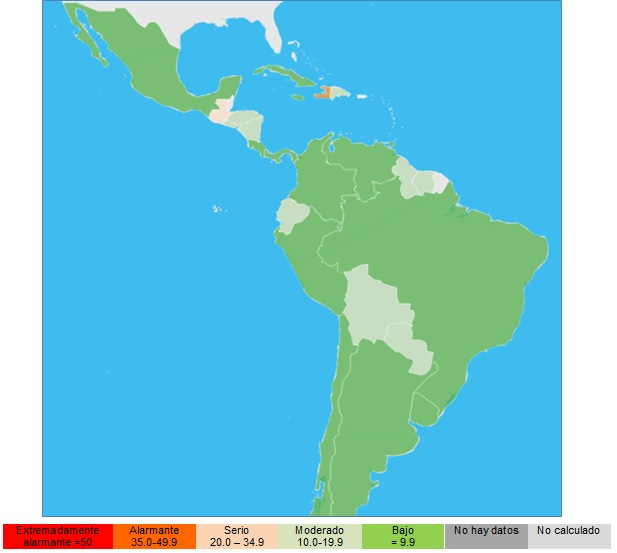
\includegraphics[width=0.7\textwidth]{figura2}
	\caption{Índice del Hambre Global para Guatemala. \textbf{Fuente:} Modificado de Ifpri, 2015.}
	\label{figura2}
\end{figure}


Como un movimiento nacional y un compromiso del Estado de Guatemala para afrontar el problema del hambre en el país, el Gobierno de Guatemala y representantes de todos los sectores firmaron el Pacto Hambre Cero en 2012 (Gobierno de Guatemala, 2012). 

Los objetivos del Pacto Hambre Cero son: «a) Reducir en 10\% la prevalencia de la desnutrición crónica infantil, para finales del 2015, promoviendo el desarrollo infantil temprano; b) prevenir el hambre estacional y reducir la mortalidad en la niñez menor de 5 años, por la desnutrición aguda; c) promover la seguridad alimentaria y nutricional, fundamento del desarrollo integral de toda la población guatemalteca, y d) prevenir y atender las emergencias alimentarias, relacionadas con el cambio climático y los desastres naturales» (Gobierno de Guatemala, 2012). 


\noindent\textbf{3.	Importancia de la estadística en seguridad alimentaria y nutricional}

A nivel mundial, existe una iniciativa para el desarrollo de la Estrategia Global para el mejoramiento de las estadísticas agrícolas y rurales (Gsars) liderada por FAO, la cual surge como una respuesta para abordar la falta de capacidad de los países en desarrollo de proporcionar datos estadísticos confiables sobre alimentación y agricultura, así como ofrecer un modelo de sistemas estadísticos agrícolas sostenible a largo plazo. Dicha estrategia está conformada por tres pilares: a) establecer un conjunto mínimo de datos básicos; b) integrar la agricultura en el sistema nacional de estadística, y c) mejorar la gobernanza y la creación de capacidad estadística (Global Strategy, 2015).
